\section{Automating Metadata Acquisition}
%
%-building names dirty -> we need some way to characterize them
%-learn
%-input output example
%-who will generate these - maybe building manager, maybe users
%-ease of use as opposed to people writing regular expressoin themselves.
%-why not have someone write the regex expressions for those most common sensors ? because people who know are not the people who use the data. building managers know, people working closely with a sensor deployment know. Sometimes the regex might get complex ...... for instanct, when is a particular tag applicable ? 
%
%Why is it this way ?

In this section, we go into detail about how we apply program synthesis techniques and the input-output model of interaction to extract enough information from sensor names to enable sufficient coverage of sensor applications. We first introduce some basic terminology we will be using throughout this section, followed by an overview of the synthesis technique in Section~\ref{sec:synth}. We then describe how we adapt the technique to the context of sensor name qualification in Section~\ref{sec:adapt}.  We finally evaluate our adapted technique on our testbed in Section~\ref{sec:eval}.

%As explained earlier, most sensor names ( or SCADA\footnote{Supervisory Control and Data Acquisition} tags ) try to encode some level of semantic information. These names might have been generated by the individual who was in charge of commissioning a building, or by following a set of vendor-specific rules. In either case, the encoded sensor names convey very little meaning to people who are not familiar with the building layout.
%
%A lot of the sense points contained in a particular building is very site-specific, e.g a building may contain a fault detector for its backup chiller, for which there might not be a well-defined sensor labelling schema from the vendor. In such scenarios, the agent commissioning a building tries his best to convey the information by using indicative labels. E.g we encountered points labelled \texttt{BLDA4S18SASA\_M}, which denotes an alarm if the supply air temperature setpoint for a supply fan gets too high\footnote{The point is to be read thus : the building name is denoted by {\it BLD}, {\it A4} indicates an air handling unit whose identification number if $4$. {\it S$18$} denotes a supple fan whose identification number if $18$, and {\it SASA\_M} denotes a supply alarm setpoint}. 

\subsection{Terminology}

The expert is expected to point out \emph{(Tag Name, Tag Value, Value Type)} tuples in the sensor name. A {\it tag} is mapped on to a substring of the sensor name, which is called its {\it value}. A tag can have a constant or a variable value. A value should be regarded a constant if it is not specific to that particular sensor. 

{\it Sample Input:} Suppose the expert is presented with an example \texttt{BLDA1R465\_\_ART}, he should qualify it in order as

 \texttt{BLDA1R465\_\_ART} : (site, \texttt{BLD}, const), (ahu, \texttt{A}, const), (ahuRef,\texttt{1}, var), (zone,\texttt{R}, const), (zoneRef, \texttt{465}, var), (zone air temp sensor, \texttt{ART}, const). 

In this example the {\bf site} tag's value is \texttt{BLD}, which is not specific to that particular sensor. Hence, the expert should mark it as a constant. On the other hand, the value of the {\bf ZoneRef} tag is specific to that sensor, and hence should be marked as variable.

{\it Sample Output:} The synthesis technique should then be able to identify the tags in a new sensor name automatically. For example, given the sensor name \texttt{BLDA5R234\_\_\_ART}, it should output the set of tuples shown below:

\texttt{BLDA5R234\_\_\_ART} : (site, \texttt{BLD}), (ahu,\texttt{A}), (ahuRef,\texttt{5}), (zone,\texttt{R}), (zoneRef,\texttt{465}), (zone air temp sensor,\texttt{ART}).

We term each of these tuples as a {\it qualification}, because it qualifies a set of alphanumeric characters into normalized metadata tags. We term the output as a {\it full qualification}, if every alphanumeric character in the sensor name was {\it qualified} by the set of outputed {\it tags}.


\subsection{Synthesis technique overview}
\label{sec:synth}

\begin{figure}[h!]
  
  \centering
    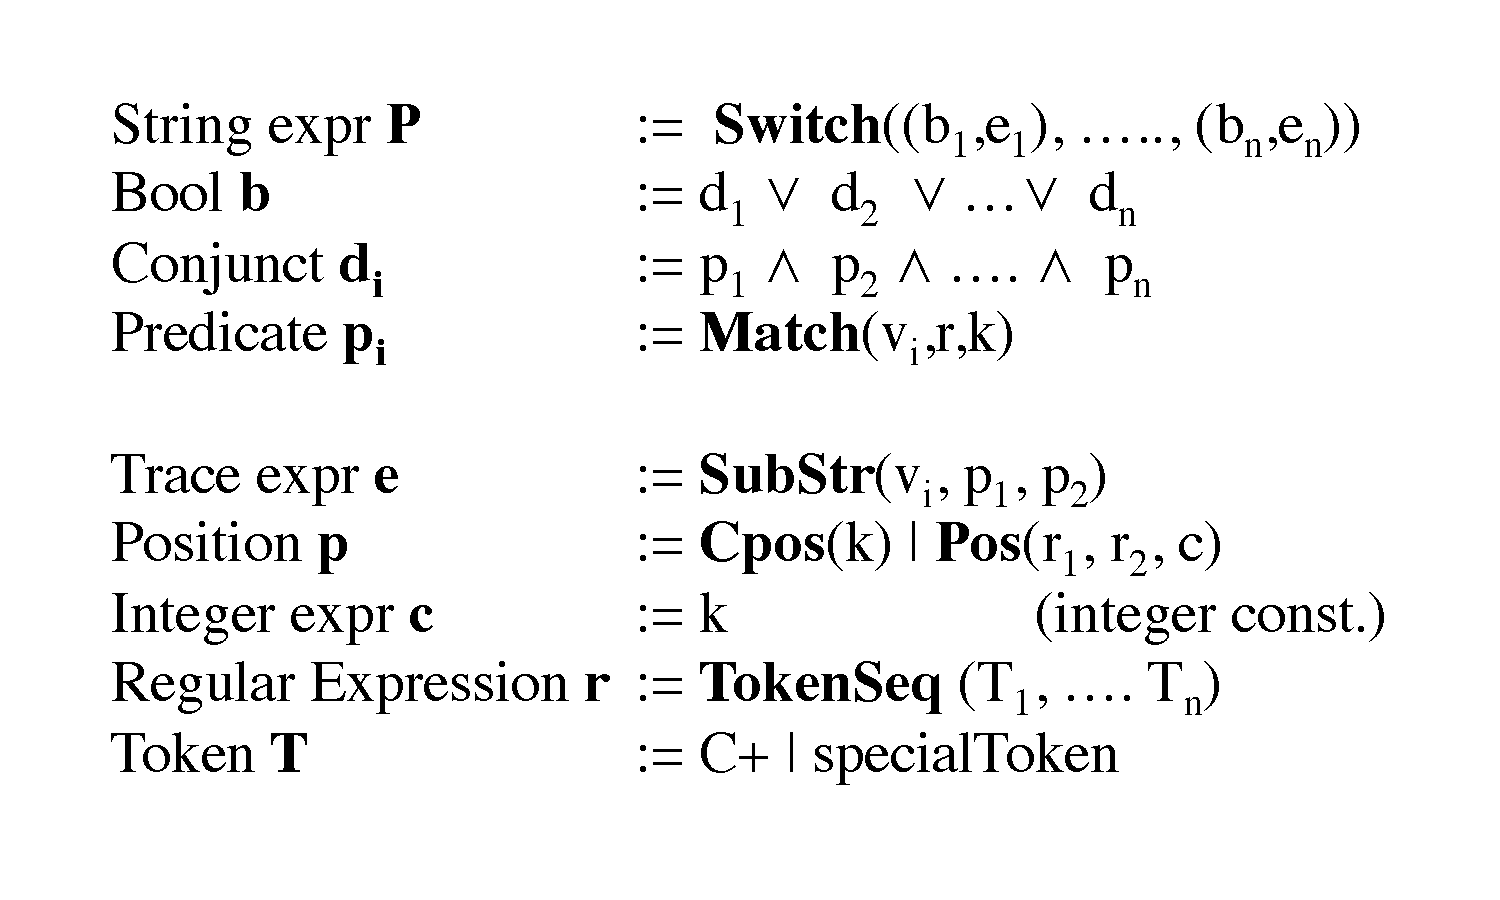
\includegraphics[width=0.5\textwidth]{figs/stringLanguage.pdf}
\caption{Language for learning substring extraction}
\label{fig:language}
\end{figure}


In this section, we will first describe the high-level logic of the synthesis technique in ~\cite{gulwani} which synthesizes simple regular expressions to transform input columns of a desired spreadsheet to a desired output column. We will then describe the set of specific techniques to adapt this to our context. 

{\bf The Algorithm:}

The main aim of the technique is to learn two sets of information from the inputed examples --- (a) whether a string transformation is applicable on a particular input, and (b) what is the set of regular expressions that transform the input string to the output string.

From each user-provided example, the set of all expressions from the language (shown in Figure~\ref{fig:language}), that could extract the required substring from that input is computed. If there are multiple input-output examples, the substring extraction rules of the multiple examples are intersected to obtain a more concise set of expressions. If the extraction expression sets cannot be intersected, they are maintained as two disjoint sets, which we shall hereby term as a {\it partitions}. 

Finally, for each disjoint set of extraction expressions, a boolean classifier is built in the DNF form, to differentiate the examples in one partition to examples in all other partitions. When a new string is given to this tool, the classifier is applied on it to figure out which partition the new input falls into, and the corresponding set of transformation expressions are then applied on it.

{\bf The Language:}

The top level expression of the language is the classifier --- the {\bf Switch}$(b_i,e_i)$ function, which applies the substring expression $e_i$ to the input only if it matches the boolean expression $b_i$. The boolean function is in DNF form and is composed of predicates of the form {\bf Match}$(v_i,r,k)$ , which evaluates to true, iff the input $v_i$ has $k$ occurences of the regular expression $r$.

The Substring expression {\bf SubStr}$(v_i,p_1,p_2)$, evaluates to the substring between positions $p_1$ and $p_2$ of the string $v_i$. {\bf CPos}$(k)$ denotes the position $k$ in the substring. A position expression {\bf pos}$(r_1,r_2,c)$ when applied on a string $s$ evaluates to a position $t$ in the subject string $s$ such that $r_1$ matches some suffix $s[0 ..t]$ and $r_2$ matches some prefix of $s[t ... l]$ (where $l$ = Length$(s)$). Also, $t$ is the $c$th such match starting from the left end of the string. The regular expressions are either just a single token $\tau$, or a token sequence, {\bf TokenSequence}$(\tau_1 .. \tau_n)$, or $\epsilon$ (which matches the empty string). The tokens $\tau$ range over some token classes, e.g one token for alphabetic characters, one for numeric characters, and one for each special character. 

We provide a couple of examples to elucidate how this technique works. 

{\bf Example 1}:

Consider, again, the sensor name \texttt{BLDA1R465\_\_ART}. The substring \texttt{ART} can be obtained, among other expressions, by either of the following language transformations :  SubString$(s, $ Cpos$(11)$, Cpos$(14))$, or SubString$(s,$ Pos(UnderscoreToken, AlphToken,$1$), Pos(AlphToken,$\epsilon, 1))$.

{\bf Example 2}: 

Suppose the synthesis algorithm has seen two examples \texttt{BLDA1R465\_\_ART}, whose desired output is \texttt{A} at index 3,  and \texttt{BLD\_\_R479\_ART}, whose desired output is \texttt{479}. One of the possible expressions that the synthesis algorithm can come up with is : Switch($(b_1, e_1), (b_2,e_2)$, where $b_1 =$ Match($s$, AlphToken UnderscoreToken,$1$), $e_1=$ Substring($s$, Cpos(3), Pos(AlphToken, NumToken,1)), and $b_2=$ Match($s$, UnderscoreToken AlphToken, 2) and $e_2$ = SubString ($s$, Cpos(6), Cpos(9)).

In general, there can be many expressions in the defined language that can obtain the desired substring, and provide a classifier to specify which types of inputs each type of substring extraction should work on.

%
%{\bf Example:} 
%
%\begin{list}
%\item example 1
%\item example 2
%
%\end{list}

\subsection{Adapting to our context}
\label{sec:adapt}

The intuition behind adapting this synthesis technique to our context is that we can consider each {\it tag} as a potential output for a given sensor name. From each given example and for each tag in that example, we can compute the set of all expressions from the language that could extract the required substring from that sensor name. Also, such a technique could learn a boolean classifier such that all tags that are present in the example evaluate their {\bf Match} condition on this example to True, and all the tags that are not, evaluate theirs to be False.

If the same tag is present in multiple examples, the tag's new extraction expression is the intersection of it's extraction expression sets for each of those examples. This may result in disjoint {\it partitions} for each tag. Finally, a boolean classifier is built to differentiate examples of each partition from all other provided examples. 

However, directly adapting this technique to the sensor naming runs into problems. We conducted an experiment where we provided examples for sensor names in a building containing 1585 sense points, applying the technique with no adaptation. Sensor names were chosen at random from the corups of all sensor names, and a full qualification of it was provided as the next input. Figure~\ref{fig:simpleTokenNoCoverage} shows the result of our experiment.

We would expect the percentage of sensor names to increase with each added example. We find this trend up to around 25 examples, after which the synthesis technique started adding qualifying substrings of the sensor name to erroneous tags. At closer inspection, it turns out that the tokens  (one for alphabetic characters, one for numeric characters, and one for each special character) used by the regular expressions and the {\bf Match} predicates were not expressive enough to capture the difference of applicability of different tags. 

To illustrate the problem, consider the examples 

{\it Example 1} : \texttt{BLDA4S1831\_STA} : [ (site, \texttt{BLD}, const), (ahu, \texttt{A}, const), (ahuRef,\texttt{4}, var), (supply fan,\texttt{S}, const), (supply fanRef,\texttt{1831}, var), (status point,\texttt{STA},const) ] ; and 

{\it Example 2}: \texttt{BLDA3R5871\_VAV} : [ (site, \texttt{BLD}, const), (ahu, \texttt{A}, const), (ahuRef, \texttt{3}, var), (zone, \texttt{R}, const), (zoneRef, \texttt{5871}, var), (vav, \texttt{VAV}, const) ]

Both these sensor names have the exact same arrangement of numeric and alphabetic characters, and special symbols, and no regular expression used by {\bf Match}$(v_i,r,c)$  would be able to discern between the two. The result would either be both tags being mapped to the same substring in an effort to qualify it, or neither. Hence, we modify the existing language and set of tokens to stay general enough, yet be more expressive.

\begin{figure}[h!]
  
  \centering
    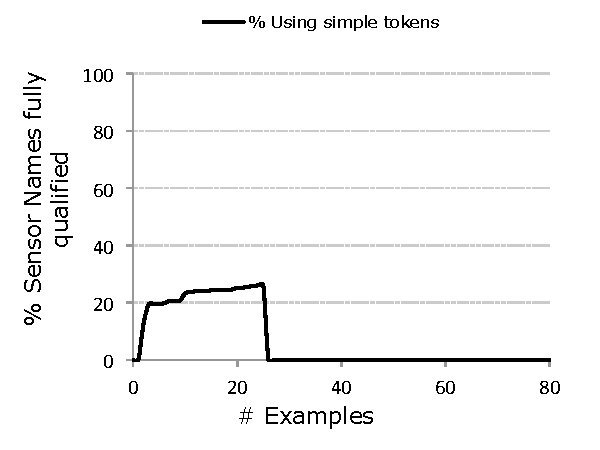
\includegraphics[width=0.5\textwidth]{figs/gulwani-noconverge.pdf}
\caption{Number of sensor names fully qualified with a token set consisting simply of alphabetic characters [A-Z], numerals [0-9], and one token for each special character.}
\label{fig:simpleTokenNoCoverage}
\end{figure}

\subsubsection{Challenges}

Adaptation of the synthesis technique to our context involves certain challenges. First, the number of tags required to fully qualify an entire building might be large, wheras certain tags may be applicable on a very limited number of sensor names. In such a case, the {\bf Match}$(v_i,r,c)$ expression for each tag should be expressive enough to differentiate a small group of sensor names from the remaining. 

Second, care should be taken while merging the {\bf SubString} rules for each tag. 

Second, a building may have 1000s of sensor points, making visual inspection of correctness of sensor name qualification very hard. Incorrectly qualification of sensor names can be mitigated by being more conservative with the boolean preciates in the top level {\bf Switch} operator. 

Below, we list five techniques that augment the basic language shown in Figure~\ref{fig:language} to enable correct classification 

\subsubsection{Token Set}

Different conventions of sensor naming from building to building precludes us from having an a priori set of special tokens to increase the effectiveness of our regular expressions. The new tokens need to be general enough Hence, we utilize  each constant tag value in the examples provided by the expert as different tokens, in addition to the normal tokens described above. 

\subsubsection{Splitting constant tags}

It may happen that a tag has multiple constant values for different points in the same building. For instance, in our test building, the {\it zone} tag was applicable either as the constant character \texttt{R} or the constant character \texttt{C}. We treat the same tags which maybe represented by two different constant string to be two different tags altogether. This helps in building better classifiers for the tags.

\subsubsection{Modifying Boolean Classifiers}

Since manual inspection of the qualification of all the points is not feasible, we take steps to strengthen the boolean classifiers corresponding to each tag. We implement different strategies for tags that have constant and variable values. If a tag has a constant value, we ensure that each clause in the DNF expression used by the {\bf Switch} operator has existence of the constant value in the sensor name as the first boolean {\bf Match} operator. This ensures that if a tag is evaluated to be applicable on a string, it has some chance of extracting the correct substring. 

Also, in cases where a tag which has a variable value, and is a reference to another tag with a constant value which is applicable on the same string, we mandate that the constant tag also have been deemed applicable on the same sensor name. For instance, in the example \texttt{BLDA1465\_ART}, the tag {\bf zoneRef} which maps to \texttt{465} has an indicator tag {\bf zone} which has a constant value. Thus, we would only evaluate the {\bf Match} expressions for {\bf zoneRef} iff the the {\bf Match} condition for the {\bf zone} tag has also evaluated to true. 




\subsubsection{Modifying Matching expression}
To make the classifiers more general, so that regular expressions learnt for one building may be applicable to sensor names of other buildings with a similar naming convention, we augment the language to include Match arguments where it evaluates to true iff the regular expression is satisfied at position equal to k. For instance, a building could be labelled ANV, and the expression learnt for air handler would not work because the token A will be matched more than once. 





%We make four design decisions to adapt the algorithm to our setting. First, we augment the set of tokens that regular expressions normally use (one token denoting an alphabetic character, one token denoting a numeric character, and a separate token for each special character), to include one token for each constant value indicated by the expert. We did this because using the non-augmented token set is not expressive enough to extract the desired substrings (as will be shown in Figure~\ref{}). Second, 
%

%Second, instead of optimizing for the minimum number of partitions that describe a tag's string extraction rules over all inputed examples, we choose an online approach which just greedily intersects the string extraction expressions from a new example with the existing partition with which it has the maximum overlap. 
%This is done to minimize overhead in an online setting , where the number of existing examples might be large ( it takes more than 100 examples to fully qualify all the sensor names on the buildings we tested our technique on ). 
%
%
%\subsection{Our adaptation}
%
%The high-level logic of our algorithm is adapted from ~\cite{gulwani}, which implemented learning simple regular expressions to transform input columns to a desired output column in a spreadsheet. The main aim of the technique is to learn two sets of information from the inputed examples --- (a) whether a particular tag is applicable on a particular sensor name, and (b) what is the set of regular expression which will give it the alpphanumeric characters corresponding to that tag. 
%
%From each expert-provided example and for each tag in that example, we compute the set of all expressions from our language (shown in Figure~\ref{language}), that could extract the required substring from that sensor name. The language defines the rules to apply regular expressions to extract required substrings from a string. If the same tag is present in more than one example, the tag's new extraction expression is the intersection of it's the extraction expression sets  for each of those examples. If the extraction expression sets cannot be intersected, they are maintained as two disjoint sets, which we shall hereby term as a {\it partitions}. The intuition behind intersecting the extraction expression sets is that as more examples containing a particular tag is seen, the extraction expressions get more and more concise. 
%
%Then, for each disjoint set of extraction expressions for each tag, a boolean classifier is built in the DNF form, to differentiate the examples containing that particular tag, from all the remaining examples. When a new sensor name is seen, the classifier is applied on it to check whether that tag is applicable on it, and if so, then the extraction expressions corresponding to the classifier is applied on the sensor name. 
%
%
%\subsection{final output - project Haystack}
%
%final output maybe in any form. 
%we realized going into this soon that not all tags conformed to any known schema. 
%For the general tags like room, ahu, vav we have conformed to the project haystack ones. 
%for the remainder of the points which are building specific, we just require that a person uses a consistent schema. 
%
%
%Boosting the metadata can enable better usability across buildings. The question automatically becomes which metadata space to normalize to. There are many metadata schemes devised for representing all buildings. Some of them are too specific and require heavy lifting, and some of them are too simple and do not meet the criteria of being expressive enough for the necessary facets of a building. 
%
%
%The goal is to normalize the existing metadata. 
%
%\subsection{Technique Overview}
%
%The synthesis technique is adapted from ~\cite{gulwani}, and tries to learn the regular expressions which 
%
%of our technique is to provide building-specific experts the ability to come up with ur technique tried to learn the regular expression patterns that 
%\subsection{learning by example}
%
%
%
%-The basic structure of our technique is derived from gluwani.
%-The goal is to 
%
%Our proposed technique is derived from the synthesis technique developed in ~\cite{}. In this section, we provide an overview of the technique, and then we will introduce how we adapt this technique to our problem. \\
%
%%\centerline{Atomic expr $f$ :=  \bf{SubStr}$(v_{i}, p_1, p_2)$}
%%\centerline{Position $p$ := $k$ | \bf{pos}$(r_1,r_2, c)$}
%%\centerline{Regular exp $r$ := $\epsilon$ | $\tau$ | \bf{TokenSeq}$(\tau_1 ...  \tau_n)$} 
%
%
%Atomic expr $f$ :=  {\bf SubStr}$(v_i, p_1, p_2)$ 
%
%Position $p$ := $k$ | {\bf pos}$(r_1,r_2, c)$ 
%
%Regular exp $r$ := $\epsilon$ | $\tau$ | {\bf TokenSeq} $(\tau_1 ...  \tau_n)$ \\
%
%
%
%
%As an example, consider that we have to extract \texttt{ART} from \texttt{BLDA1R465\_\_ART}, the substring expression can be written as {\bf SubStr}$(s, -3, -14)$, or {\bf SubStr}$(s,$ {\bf Pos()}
%
%
%
%
% way we learn regular expressions from inputs provided by the expert. We shall use the example scada tag {\tt BLDA1R465  ART} as a goto example throughout this section.
%
%In the following sections, we will use the word {\it token} to refer a token from a character class. So a token might be is a character or a group of characters in a point to be expanded. In the For instance, in the point {\tt BLDA1R465 ART} has the tokens as shown in Figure~\ref{fig:exampleInput}
%
%
%\subsubsection{Inputs}
%
%For every example an expert provides, we require three types of information - (a) the normalized metadata tag which is contained in the point name,  (b) the mapping of the labels in the data to normalized metadata tags , (c) the starting point of those labels, and (d) whether the value of the label is a constant or variable. For instance, consider the expert is asked to fully qualify the sensor point name \texttt{BLDA1R435\_\_ART}. Shown below is the expected input by the user.
%
%
%
%The aim of the learning algorithm would then be to fully qualify the remaining examples
%
%
%
%Whenever the expert types in the explanation for an input, we require that the expert give a full description of the point. The full description of a point consist of the haystack tags the point contains, the starting and ending position of the string that correspond to the haystack tag, mentioning whether the substring is a constant or is variable. For instance, in our example, {\tt BLD} is a constant for the haystack tag {\bf site}, but {\tt 465} is a variable substring, because the tag value will change from point to point. 
%
%
%are the tokens contained in a tag, their starting and ending positions, whether the tag has an associated value, and whether the associated value 
%
%\subsection{challenges}
%
%
%-different types of points all together in the same corpus, and it is not one or two . you have to generate a regex classifier for all known tags. 
%-tokens vary from building to building -> so no pre-defined token ( alternative were using Excel's stuff or treating every letter as an individual token ). Show the experiment that shows the number of incorrectly qualified vs number of examples added.
%-simplest classifier to more complex classifier
%
%
%
%\subsection{technique we chose and modifications}
%
%learning by input output example
%- subtring generation
%-intersection
%-predicate generation
%


\section{Evaluation of Learning By Example}
\label{sec:eval}

In this section, we guage the effectiveness of our learning by example technique by evaluating the number of examples required to qualify labels in two large commercial buildings. 

\subsection{Testbed}

We manually generated ground truth data for all the points in two buildings whose building management system was installed by different vendors. Building $1$ has 1586 sensor points and was built in the 1990s. Building $2$ was built in the 2000s and has 2551 sense points. The label characteristics of the two buildings are shown in Figure~\ref{fig:buildingLabelCharacteristics}. 

Figure~\ref{fig:labelFreq} shows that in  these two buildings, a few labels (about 20 in each building) frequently appear in a lot of sensor names. This is pretty common in commercial buildings, where a majority of the points are related to zone or room information. For instance, Building $1$, has a room setpoint sensor, an airflow sensor and temperature sensor for each of its more than 200 rooms. Each of these points have a label indicating that they are a room, and a room number. These most frequent labels also fully qualify a large number of the sensor names in both buildings. In other words, learning proper classifiers and qualifications for about 20 labels could yield a full qualification for 80\% of the sensor names in both these buildings.

The distribution frequency of labels also has a long tail. For both the buildings, the labels corresponding to {\it site} and {\it zoneRef} are most common. However, the distribution of labels show that there is also a long tail. These comprise of building specific sensors, alarms or status variables. There are also a lot of incomplete or inconsistent labeling of sensor names, the labels of which fall in this long tail. Thus, one of the main objectives of the learning algorithm is that it does not learn wrong classifiers for labels based on sensor names that fall in this long tail.

\begin{figure}[h!]]
\centering
	\begin{subfigure}{0.48\textwidth}
                \centering
		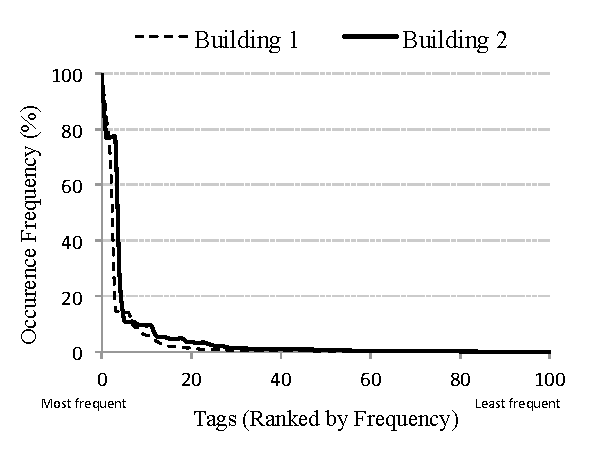
\includegraphics[width=\textwidth]{./figs/pointOccuranceFreq.pdf}
                \caption{Percentage of sensor names each label appears in. The x-axis is sorted according to the frequency of occurence of a label}
                \label{fig:labelFreq}
	\end{subfigure}
	\begin{subfigure}{0.48\textwidth}
                \centering
		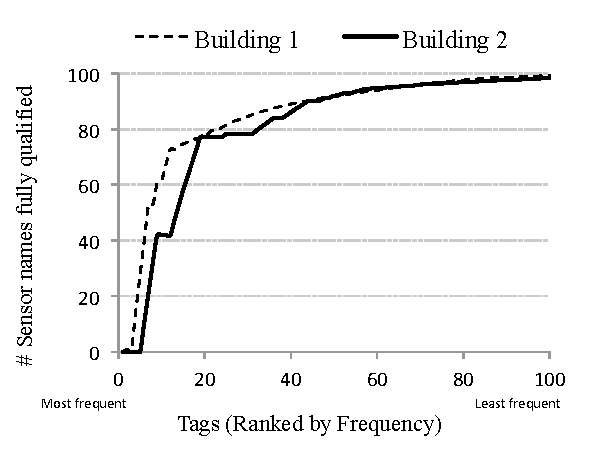
\includegraphics[width=\textwidth]{./figs/pointCDF.pdf}
                \caption{Percentage of sensor names fully qualified by the highest ranking labels. A point ($x$,$y$) indicates that $y$ sensor names could be fully qualified by using labels ranked $1$ ... $x$}
                \label{fig:pointCDF}
	\end{subfigure}
\caption{Characteristics of labels from two buildings we generated ground-truth data to test our learning technique}
\label{fig:buildingLabelCharacteristics}
\end{figure}



\subsection{Choosing the Next Example}


The large number of sensors in a building pose a challenge in selecting the next example to present to the expert. First, the expert might not always be able to browse through all sensor points to check correct qualification. Also, an expert might visally not be able to discern which points would add the most amount of information to the learning process. 

This process can be facilitated by the internal notion the learning algorithm has of how much of each sensor name it has been able to qualify. This notion is maintained by simply comparing the sensor name to all the labels that the algorithm applied on it. Note that, the algorithm can incorrectly apply labels on a sensor name, which may lead to erroneous conclusions. The incorrect application of labels might be due to incorrectness or incompleteness of the boolean matching expression or the string extraction regular expressions.

We implemented four different generators to evaluate which example should be provided next to the expert:

{\bf Random:} This generator just finds at random the next example to present to the expert. While choosing the example, the random algorithm chooses among the set of sensor names which it feels it has not been able to fully qualify.  

{\bf MinRemaining :} This generator chooses the example, that according to our tool, has the minimum string length left to qualify. The intuition behind this is to gain more concrete knowledge about a small number of labels.

{\bf MaxRemaining :} This chooses the example, that the learning technique feels has the maximum string length left to qualify. These examples would help the learning technique gain coverage over the space of unsees labels. The more labels the learning technique knows, the more sensor name information it will be able to qualify.

{\bf Self-Correcting :} There are some sensor names where the learning algorithm can itself figure out that it has incorrectly qualified a sensor name. There can be three such indicators. First, for a sensor name which has matched its boolean classifier, none of its left or right position regular expressions is applicable. Second, if the sensor name has been qualified with labels that overlap over the same substring. Third, the learning algorithm can get a notion of the labelling uncertainty of a sensor name, if its qualification labels change drastically when a new example has been added. This generator gives the expert the examples that satisfy the most number of these three criteria. Once, none of the points satisfy these criteria, this generator defaults to the MinRemaining generator.


We wrote a script that automatically gave the learning algorithm the example that it asked for, and evaluated the qualifications provided by the algorithm. We terminated when the number of correct full sensor qualifications reached 70\%. Figures ~\ref{fig:active-learning} show the results of the four generators on the two buildings. The \emph{Random} generator took the least number of examples to achieve full qualification of 70\% of the sensor names, achieving it much quicker than the others. The reason for this is due to the long tail of the label distribution as was shown in Figure~\ref{}. The top 20 most occurring labels, by themselves, can fully qualify about 80\% of the sensor names. A random generator has a high probability of finding one of these 80\% of the points, thus acquanting itself more quickly of the most frequently occuring labels. Neither of the other three classifiers is able to achieve that. They get stuck trying to either get every bit of information from sensor with obscure labels (\emph{MinRemaining}), or trying to cover more labels by first qualifying sensors which have been least qualified(\emph{MaxRemaining}), or by choosing form the set of ill-formed sensor names, which would indicate errors to the learning algorithm (\emph{Self-Correcting}).

\begin{figure}[h!]
\centering
	\begin{subfigure}{0.48\textwidth}
                \centering
		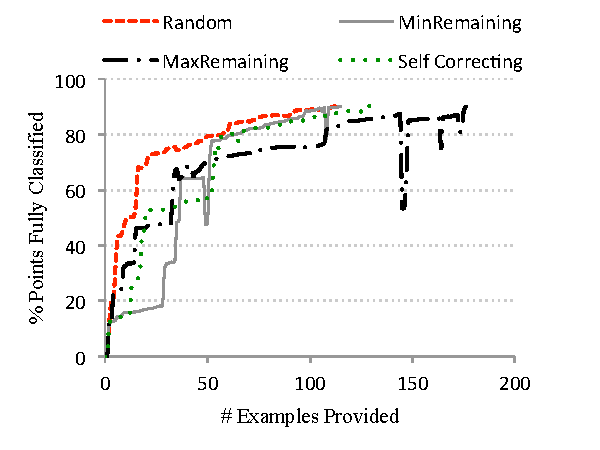
\includegraphics[width=\textwidth]{./figs/soda-active-learning.pdf}
                \caption{Building 1}
                \label{fig:active-learning-soda}
	\end{subfigure}
	\begin{subfigure}{0.48\textwidth}
                \centering
		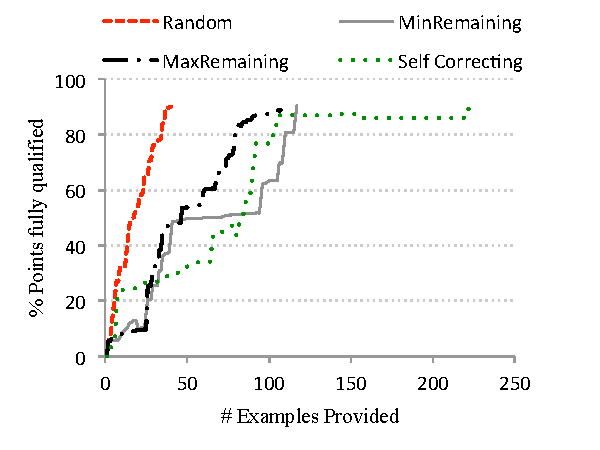
\includegraphics[width=\textwidth]{./figs/sdh-active-learning.pdf}
                \caption{Building 2}
                \label{fig:active-learning-sdh}
	\end{subfigure}
\caption{The number of examples required to fully qualify 70\% of sensor names in two buildings}
\label{fig:active-learning}
\end{figure}



\subsection{Applying to other buildings}

One of the major goals of learning from examples provided by an expert is that the learnt regular expressions may be applicable to other buildings which have similar naming conventions. In this section, we evaluate the efficacy of the regular expressions learnt on Building 1 of our testbed with the remaining 55 buildings on campus, each of which was commissioned by the same vendor. As mentioned before, the remaining buildings comprise about 15,000 sensor points.

Figure~\ref{fig:campusWideStats} shows the applicability of tags learnt from Building $1$ to the remaining buildings. Tags which were most frequent in Building $1$ such as {\bf zone, zoneRef} and {\bf ahuRef}, were also widely applicable throughout other buildings. This is expected because all these buildings are commercial offices, with a large number of zone, and a set of points associated with each zone. There are also a few tags which are infrequent in a particular building, but applicable across all buildings, e.g the {\bf return water temp} tag or the {\bf outside air temp} tag. Thus, fully qualifying even one building has the potential to yield regular expressions that can then be propagated across buildings.

It was impractical to ground truth all the buildings, and its 15,000 sensor points for our experiment. Hence, we hand wrote regular expressions to the best of our efforts to qualify sensor names in those buildings. It is this manual qualification data that we treat as ground truth in the our experiment. We use the regular expressions obtained after 90\% of the sensor points in Building $1$ was fully qualified. While running these expressions on a different building, we just replaced the token corresponding to the tag {\bf site} to the building-specific {\bf site}  token. 

Figure~\ref{fig:recallCampusWide} shows the true-positive rate based for each tag based on our ground truth data. The true positive rate indicates that the required tag was correctly applied where it was applicable, and it was able to qualify the correct substring from the corresponding sensor name. As we can see, the regular expressions were able to identify almost all the buildings that each tag learnt from Building $1$ was applicable to. Some of the tags could not be applicable to other buildings, because they use different constant values for the same tag name. For instance, the {\bf exhaust fan} tag is specified in certain buildings as \texttt{EF}, wheras in Building $1$ it was specified as \texttt{E}. Also, certain variable tags vary in format across buildings, e.g the {\bf zoneRef} tag, which leads to a lower true positive rate for such tags. 

The implications of 
 

\begin{figure}[h!]
\centering
	\begin{subfigure}{0.48\textwidth}
                \centering
		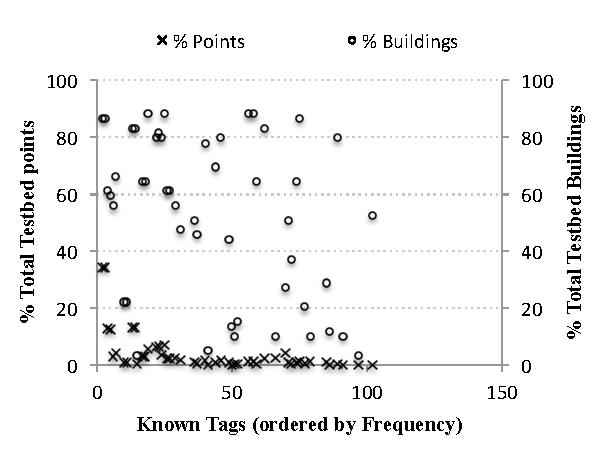
\includegraphics[width=\textwidth]{./figs/campusWideStats.pdf}
                \caption{Building 1}
                \label{fig:campusWideStats}
	\end{subfigure}
	\begin{subfigure}{0.48\textwidth}
                \centering
		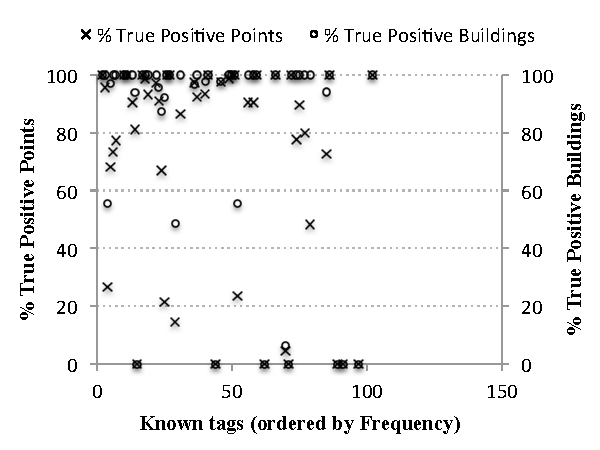
\includegraphics[width=\textwidth]{./figs/recallCampusWide.pdf}
                \caption{Building 2}
                \label{fig:recallCampusWide}
	\end{subfigure}
\caption{The number of examples required to fully qualify 70\% of sensor names in two buildings}
\label{fig:active-learning}
\end{figure}






